\documentclass{article}
\usepackage[utf8]{inputenc}
\usepackage{subcaption}
\usepackage{amsmath}
\usepackage{amssymb}
\usepackage{hyperref}
\usepackage{titlesec}
\usepackage{xcolor}
\usepackage{fancyhdr}
\usepackage{graphicx}
\usepackage{tcolorbox}
\usepackage{multirow}
\usepackage[rightcaption]{sidecap}
\usepackage{verbatim}
\usepackage[backend=bibtex]{biblatex}
\usepackage{blindtext}
\usepackage{multicol}
\usepackage [ a4paper , top = 0.8 in, hmargin = 0.8 in , bottom =0.8 in ] { geometry }
\hypersetup{
    colorlinks=true,
    linkcolor=blue,
    filecolor=magenta,      
    urlcolor=cyan,
}
\setlength\parindent{0pt}
\usepackage{enumitem}

\bibliography{bibliography}
\fancyhead[L]{CS349}
\fancyhead[R]{Project Submission Stage 1}
\fancyfoot[C]{Page \thepage}

\DeclareMathOperator*{\maxi}{max}
\DeclareMathOperator*{\mini}{min}

\graphicspath{{images/}}

\begin{document}

\title{\large{CS349: Project Submission Stage 1} \\ \Huge \textbf{XData Extensions}}
\date{}
\author{Satyankar Chandra (22B0967) \\
Ayan Tanwar (22B0931) \\
Gourish Garg (22B0915) \\
Harsh Kumar (22B0973)}
\pagestyle{fancy}

\maketitle

\section{Project Overview}

\textbf{Aim:} Extend XData to support in-browse postgresql execution using \href{https://pglite.dev/}{pglite.dev}. Make sure everything runs from local resources so it can be run for exams without external internet. This allows each user to run in their own database without accessing any central database. The next step is to extend XData system to run the queries in browser rather than on a backend database.

\section{Project Proposal}

In our initial project proposal, we aimed to extend the XData system and implement the following features:
\begin{itemize}
    \item Query Profiling and Runtime Analysis $\checkmark$
    \item Evaluation Plans and Query Optimization $\checkmark$
    \item Client Side Autograding
    \item Support for Concurrent Queries
    \item Adding Constraints to Queries
\end{itemize}

Our team has been working on all of these features in parallel. We have made significant progress on the first two features, and we are currently working on the third and fourth features. The fifth feature is still in the planning stage.

\section{Current Progress}

Below is the current status of our project for each of the features:

\subsection{Query Profiling and Runtime Analysis}

TODO Ayan

\subsection{Evaluation Plans and Query Optimization}

PostgreSQL has various options to evaluate a query. For example, for a search query (typically a \verb|SELECT| query), it can perform a \verb|Seq Scan|, \verb|Index Scan|, \verb|Bitmap Index Scan| or \verb|TID Scan|. Similarly there are multiple possibilities for \verb|JOIN|, \verb|SORT| and \verb|GROUP BY| operations. The query planner chooses the best option based on the statistics of the tables involved in the query.

\medskip

Even though PostgreSQL displays the evaluation plan for a query by using the \verb|EXPLAIN ANALYZE| command, it does not provide the option to choose a specific evaluation plan. We have implemented a feature that allows the user to choose the evaluation plan for a query. The user can select the evaluation plan for each operation in the query and compare the Planning and Execution time for different evaluation plans.

\medskip

This feature is implemented by setting the \verb|enable_*| flags in PostgreSQL. For example, to enable \verb|Seq Scan|, we set the \verb|enable_seqscan| flag to \verb|on| and all other flags to \verb|off|. This allows us to choose a specific evaluation plan for a query.

\begin{figure}[htbp]
    \centering
    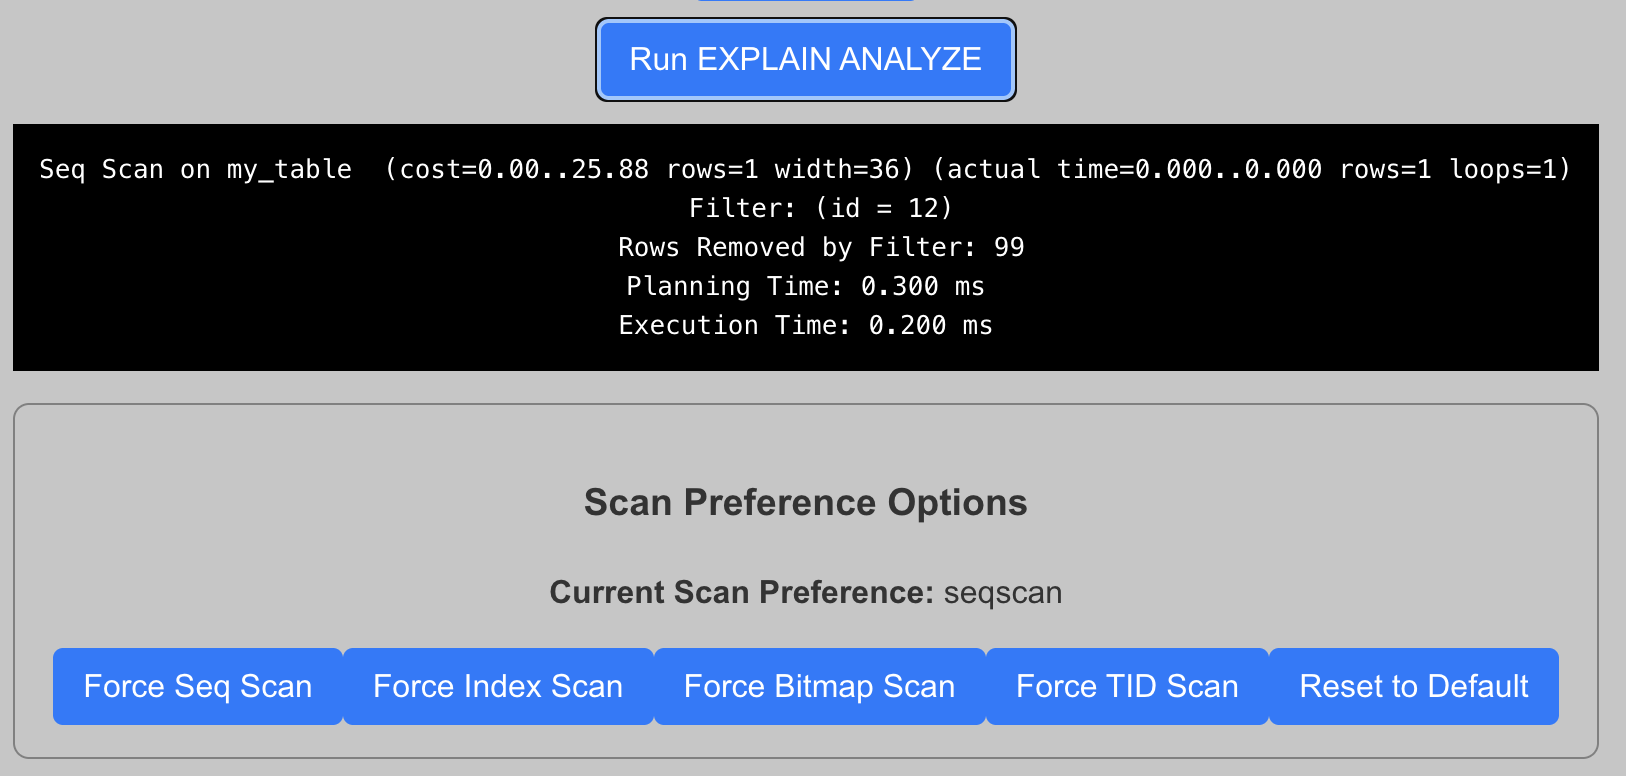
\includegraphics[width=0.8\textwidth]{seq.png}
    \caption{Selecting Sequential Scan for a query}
\end{figure}


\begin{figure}[htbp]
    \centering
    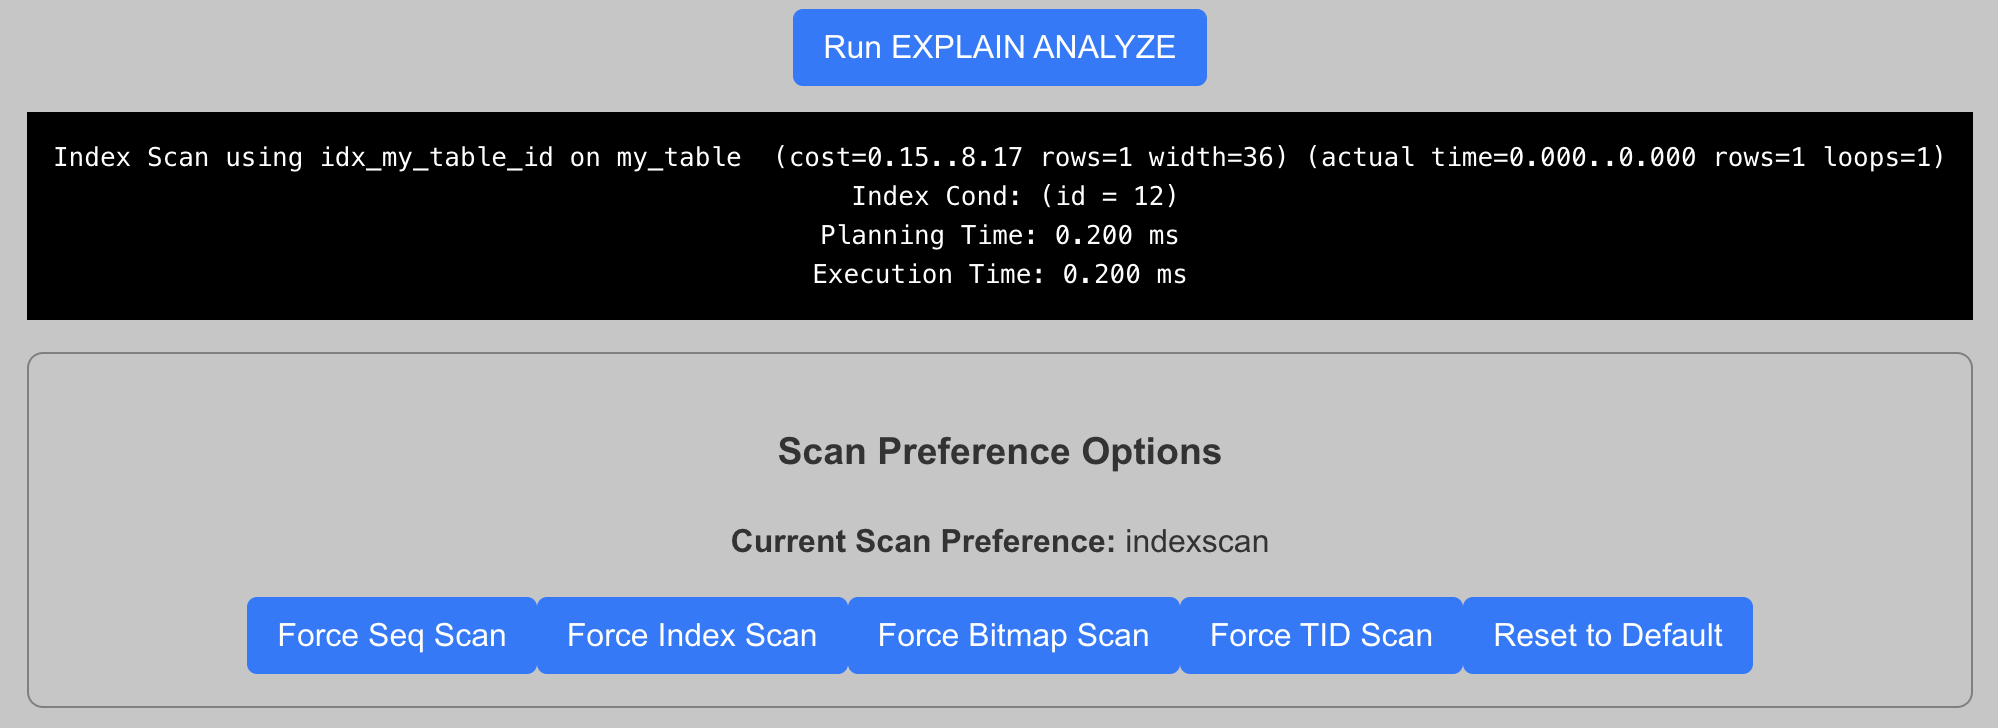
\includegraphics[width=0.8\textwidth]{index.png}
    \caption{Selecting Index Scan for a query}
\end{figure}

The main utility of this feature is that sometimes the query planner chooses a suboptimal evaluation plan for a query. This can happen if the statistics of the tables involved in the query are not up to date. In such cases, the user can look at the performance of different evaluation plans and choose the best one. This feature is useful for debugging and optimizing queries.


\subsection{Other Features}

The other 3 features are still being worked on. We have included them in our future plan of action and provided a rough timeline for their implementation.

\section{Future Plan of Action and Timeline}

The tasks remaining with their expected time to completion for the project are as follows:
\begin{itemize}
    \item \textbf{Client Side Autograding (1 Week):} Since PGLite is a client side database, we can directly run and check queries on the client side. To avoid leaking the solution, we are currently using a hash of the solution. The autograder will check the hash of the solution against the expected hash. We are also exploring the possibility of dumping the database to a file and checking the file against the expected file.
    \item \textbf{Support for Concurrent Queries (1 Week):} We are also working on supporting concurrent queries. We plan to use \verb|pg_locks| to ensure that the queries are executed in a serializable manner. This will allow us to run multiple queries at the same time without any conflicts.
    \item \textbf{Adding Constraints to Queries (2 Weeks):} We are still figuring out how to implement this feature. One approach we are trying is whitelisting operations that can be performed in a query. However, this approach is not very flexible and leads to many unwanted constraints. We are also exploring the possibility of using a query parser with a small local LLM to check the constraints.
    \item \textbf{Integration with XData Code (Last 2-3 days):} We also need to integrate our code with the XData codebase. This can be done after discussing with the XData team at the later stage of the project.
\end{itemize}


\section{Challenges Faced}
While working on the project, we faced several challenges. We already resolved some of them, but few are still pending. Some of them are:
\begin{itemize}
    \item PGLite does not provide any API to parse and view the AST for PostgreSQL queries. This makes it difficult to implement the query profiling and runtime analysis feature. We are relying on a third-party library to currently do the same.
    \item PGLite crashes with large databases. This makes it harder to observe a significant difference in the performance of different evaluation plans. We are currently working on a workaround to this issue.
    \item The documentation for PGLite is not very clear. This is especially the case for the React integration with PGLite. Although we were able to use some of the provided React Hooks for PGLite, we had to figure out the rest of the integration ourselves. 
\end{itemize}

\section{Conclusion}

In conclusion, we feel that we have made significant progress on the project. We have implemented the query profiling and runtime analysis feature, and we are also working on the other 3 features. We are very open to feedback and suggestions from the XData team in regards to the project and the features we are implementing. Our team is very enthusiastic about the project and hope that we have some meaningful contributions to the existing XData platform by the end of this semester.

    
\end{document}